% Generated by Sphinx.
\def\sphinxdocclass{report}
\documentclass[letterpaper,10pt,english]{sphinxmanual}
\usepackage[utf8]{inputenc}
\DeclareUnicodeCharacter{00A0}{\nobreakspace}
\usepackage[T1]{fontenc}
\usepackage{babel}
\usepackage{times}
\usepackage[Bjarne]{fncychap}
\usepackage{longtable}
\usepackage{sphinx}


\title{TiberCAD Theory Module}
\date{February 15, 2011}
\release{1.2.2}
\author{TiberLAB srl}
\newcommand{\sphinxlogo}{
\includegraphics{logo.png}\par}
\renewcommand{\releasename}{Release}
\makeindex

\makeatletter
\def\PYG@reset{\let\PYG@it=\relax \let\PYG@bf=\relax%
    \let\PYG@ul=\relax \let\PYG@tc=\relax%
    \let\PYG@bc=\relax \let\PYG@ff=\relax}
\def\PYG@tok#1{\csname PYG@tok@#1\endcsname}
\def\PYG@toks#1+{\ifx\relax#1\empty\else%
    \PYG@tok{#1}\expandafter\PYG@toks\fi}
\def\PYG@do#1{\PYG@bc{\PYG@tc{\PYG@ul{%
    \PYG@it{\PYG@bf{\PYG@ff{#1}}}}}}}
\def\PYG#1#2{\PYG@reset\PYG@toks#1+\relax+\PYG@do{#2}}

\def\PYG@tok@gd{\def\PYG@tc##1{\textcolor[rgb]{0.63,0.00,0.00}{##1}}}
\def\PYG@tok@gu{\let\PYG@bf=\textbf\def\PYG@tc##1{\textcolor[rgb]{0.50,0.00,0.50}{##1}}}
\def\PYG@tok@gt{\def\PYG@tc##1{\textcolor[rgb]{0.00,0.25,0.82}{##1}}}
\def\PYG@tok@gs{\let\PYG@bf=\textbf}
\def\PYG@tok@gr{\def\PYG@tc##1{\textcolor[rgb]{1.00,0.00,0.00}{##1}}}
\def\PYG@tok@cm{\let\PYG@it=\textit\def\PYG@tc##1{\textcolor[rgb]{0.25,0.50,0.56}{##1}}}
\def\PYG@tok@vg{\def\PYG@tc##1{\textcolor[rgb]{0.73,0.38,0.84}{##1}}}
\def\PYG@tok@m{\def\PYG@tc##1{\textcolor[rgb]{0.13,0.50,0.31}{##1}}}
\def\PYG@tok@mh{\def\PYG@tc##1{\textcolor[rgb]{0.13,0.50,0.31}{##1}}}
\def\PYG@tok@cs{\def\PYG@tc##1{\textcolor[rgb]{0.25,0.50,0.56}{##1}}\def\PYG@bc##1{\colorbox[rgb]{1.00,0.94,0.94}{##1}}}
\def\PYG@tok@ge{\let\PYG@it=\textit}
\def\PYG@tok@vc{\def\PYG@tc##1{\textcolor[rgb]{0.73,0.38,0.84}{##1}}}
\def\PYG@tok@il{\def\PYG@tc##1{\textcolor[rgb]{0.13,0.50,0.31}{##1}}}
\def\PYG@tok@go{\def\PYG@tc##1{\textcolor[rgb]{0.19,0.19,0.19}{##1}}}
\def\PYG@tok@cp{\def\PYG@tc##1{\textcolor[rgb]{0.00,0.44,0.13}{##1}}}
\def\PYG@tok@gi{\def\PYG@tc##1{\textcolor[rgb]{0.00,0.63,0.00}{##1}}}
\def\PYG@tok@gh{\let\PYG@bf=\textbf\def\PYG@tc##1{\textcolor[rgb]{0.00,0.00,0.50}{##1}}}
\def\PYG@tok@ni{\let\PYG@bf=\textbf\def\PYG@tc##1{\textcolor[rgb]{0.84,0.33,0.22}{##1}}}
\def\PYG@tok@nl{\let\PYG@bf=\textbf\def\PYG@tc##1{\textcolor[rgb]{0.00,0.13,0.44}{##1}}}
\def\PYG@tok@nn{\let\PYG@bf=\textbf\def\PYG@tc##1{\textcolor[rgb]{0.05,0.52,0.71}{##1}}}
\def\PYG@tok@no{\def\PYG@tc##1{\textcolor[rgb]{0.38,0.68,0.84}{##1}}}
\def\PYG@tok@na{\def\PYG@tc##1{\textcolor[rgb]{0.25,0.44,0.63}{##1}}}
\def\PYG@tok@nb{\def\PYG@tc##1{\textcolor[rgb]{0.00,0.44,0.13}{##1}}}
\def\PYG@tok@nc{\let\PYG@bf=\textbf\def\PYG@tc##1{\textcolor[rgb]{0.05,0.52,0.71}{##1}}}
\def\PYG@tok@nd{\let\PYG@bf=\textbf\def\PYG@tc##1{\textcolor[rgb]{0.33,0.33,0.33}{##1}}}
\def\PYG@tok@ne{\def\PYG@tc##1{\textcolor[rgb]{0.00,0.44,0.13}{##1}}}
\def\PYG@tok@nf{\def\PYG@tc##1{\textcolor[rgb]{0.02,0.16,0.49}{##1}}}
\def\PYG@tok@si{\let\PYG@it=\textit\def\PYG@tc##1{\textcolor[rgb]{0.44,0.63,0.82}{##1}}}
\def\PYG@tok@s2{\def\PYG@tc##1{\textcolor[rgb]{0.25,0.44,0.63}{##1}}}
\def\PYG@tok@vi{\def\PYG@tc##1{\textcolor[rgb]{0.73,0.38,0.84}{##1}}}
\def\PYG@tok@nt{\let\PYG@bf=\textbf\def\PYG@tc##1{\textcolor[rgb]{0.02,0.16,0.45}{##1}}}
\def\PYG@tok@nv{\def\PYG@tc##1{\textcolor[rgb]{0.73,0.38,0.84}{##1}}}
\def\PYG@tok@s1{\def\PYG@tc##1{\textcolor[rgb]{0.25,0.44,0.63}{##1}}}
\def\PYG@tok@gp{\let\PYG@bf=\textbf\def\PYG@tc##1{\textcolor[rgb]{0.78,0.36,0.04}{##1}}}
\def\PYG@tok@sh{\def\PYG@tc##1{\textcolor[rgb]{0.25,0.44,0.63}{##1}}}
\def\PYG@tok@ow{\let\PYG@bf=\textbf\def\PYG@tc##1{\textcolor[rgb]{0.00,0.44,0.13}{##1}}}
\def\PYG@tok@sx{\def\PYG@tc##1{\textcolor[rgb]{0.78,0.36,0.04}{##1}}}
\def\PYG@tok@bp{\def\PYG@tc##1{\textcolor[rgb]{0.00,0.44,0.13}{##1}}}
\def\PYG@tok@c1{\let\PYG@it=\textit\def\PYG@tc##1{\textcolor[rgb]{0.25,0.50,0.56}{##1}}}
\def\PYG@tok@kc{\let\PYG@bf=\textbf\def\PYG@tc##1{\textcolor[rgb]{0.00,0.44,0.13}{##1}}}
\def\PYG@tok@c{\let\PYG@it=\textit\def\PYG@tc##1{\textcolor[rgb]{0.25,0.50,0.56}{##1}}}
\def\PYG@tok@mf{\def\PYG@tc##1{\textcolor[rgb]{0.13,0.50,0.31}{##1}}}
\def\PYG@tok@err{\def\PYG@bc##1{\fcolorbox[rgb]{1.00,0.00,0.00}{1,1,1}{##1}}}
\def\PYG@tok@kd{\let\PYG@bf=\textbf\def\PYG@tc##1{\textcolor[rgb]{0.00,0.44,0.13}{##1}}}
\def\PYG@tok@ss{\def\PYG@tc##1{\textcolor[rgb]{0.32,0.47,0.09}{##1}}}
\def\PYG@tok@sr{\def\PYG@tc##1{\textcolor[rgb]{0.14,0.33,0.53}{##1}}}
\def\PYG@tok@mo{\def\PYG@tc##1{\textcolor[rgb]{0.13,0.50,0.31}{##1}}}
\def\PYG@tok@mi{\def\PYG@tc##1{\textcolor[rgb]{0.13,0.50,0.31}{##1}}}
\def\PYG@tok@kn{\let\PYG@bf=\textbf\def\PYG@tc##1{\textcolor[rgb]{0.00,0.44,0.13}{##1}}}
\def\PYG@tok@o{\def\PYG@tc##1{\textcolor[rgb]{0.40,0.40,0.40}{##1}}}
\def\PYG@tok@kr{\let\PYG@bf=\textbf\def\PYG@tc##1{\textcolor[rgb]{0.00,0.44,0.13}{##1}}}
\def\PYG@tok@s{\def\PYG@tc##1{\textcolor[rgb]{0.25,0.44,0.63}{##1}}}
\def\PYG@tok@kp{\def\PYG@tc##1{\textcolor[rgb]{0.00,0.44,0.13}{##1}}}
\def\PYG@tok@w{\def\PYG@tc##1{\textcolor[rgb]{0.73,0.73,0.73}{##1}}}
\def\PYG@tok@kt{\def\PYG@tc##1{\textcolor[rgb]{0.56,0.13,0.00}{##1}}}
\def\PYG@tok@sc{\def\PYG@tc##1{\textcolor[rgb]{0.25,0.44,0.63}{##1}}}
\def\PYG@tok@sb{\def\PYG@tc##1{\textcolor[rgb]{0.25,0.44,0.63}{##1}}}
\def\PYG@tok@k{\let\PYG@bf=\textbf\def\PYG@tc##1{\textcolor[rgb]{0.00,0.44,0.13}{##1}}}
\def\PYG@tok@se{\let\PYG@bf=\textbf\def\PYG@tc##1{\textcolor[rgb]{0.25,0.44,0.63}{##1}}}
\def\PYG@tok@sd{\let\PYG@it=\textit\def\PYG@tc##1{\textcolor[rgb]{0.25,0.44,0.63}{##1}}}

\def\PYGZbs{\char`\\}
\def\PYGZus{\char`\_}
\def\PYGZob{\char`\{}
\def\PYGZcb{\char`\}}
\def\PYGZca{\char`\^}
\def\PYGZsh{\char`\#}
\def\PYGZpc{\char`\%}
\def\PYGZdl{\char`\$}
\def\PYGZti{\char`\~}
% for compatibility with earlier versions
\def\PYGZat{@}
\def\PYGZlb{[}
\def\PYGZrb{]}
\makeatother

\begin{document}

\maketitle
\tableofcontents
\phantomsection\label{index::doc}



\chapter{Thermal}
\label{Thermal:thermal}\label{Thermal::doc}\label{Thermal:welcome-to-tibercad-s-documentation}\label{Thermal:contents}\label{Thermal:id1}

\chapter{Elasticity}
\label{Elasticity::doc}\label{Elasticity:elasticity}\label{Elasticity:id1}

\section{Abstract}
\label{Elasticity:abstract}
Elasticity? is a Finite Elements solver for mechanical equilibrium problems.
It brings features typically developed for structural stability solvers into device modeling.
The coupled treatment of the electro-mechanical problem within a unique framework results very useful to explore for multidisciplinary ideas.



\section{Mini theoretical intro}
\label{Elasticity:mini-theoretical-intro}
Assuming a small displacement, Elasticity? elasticity computed the strain by solving the equation

\[
\frac{\partial}{\partial x_j}C_{ijlk}\frac{\partial u_l}{\partial x_k} = f_i
\]
where C is the stiffness constant  and f is the total external body force.
The latter may include several contribution such as the converse piezoelectric effect the thermal expansion and a lattice mismatch induced strain.
The latter, described in the example below, occurs when an interface is created between two materials with different lattice constants.
Let $\epsilon^{LM}$ be the lattice mismatch strain, then the effective body force reads as :

 \[
 f_i = -\frac{\partial }{\partial x_j} C_{ijlk}\epsilon_{lk}^{LM}
 \]

\section{Example}
\label{Elasticity:example}
In the following we will compute the strain induced by the lattice mismatch in a system comprising a layer of GaN between two contacts of $Al_{x}Ga_{1-x}N$ .
Once the mesh is created with gmsh (distributed along TiberCAD?) we may start to build the input file.
First, we have to insert the region section


\begin{Verbatim}[commandchars=@\[\]]
Device
  {
   dimension = 3
   meshfile = mesh.msh
   mesh@_units = 1e-9
   material = AlGaN
   x = 0.2
   x-growth-direction = (-1,0,1,0)
   y-growth-direction = (-1,2,-1,0)
   z-growth-direction = (0,0,0,1)
   Region Well  {material = GaN}
  }
\end{Verbatim}

All the options included in this section, such ad the material, axis growth and alloy concentration, apply for the whole structure.
If we want to specify a region with different properties, we may use the keyword Region and refer to a region name, as specified in the mesh file.


The second part of the input file is devoted to the module declaration


\begin{Verbatim}[commandchars=@\[\]]
Module elasticity
  {
   Physics
     {
      BodyForcelattice@_mismatch
        {
         x-growth-direction = (-1,0,1,0)
         y-growth-direction = (-1,2,-1,0)
         z-growth-direction = (0,0,0,1)
         reference@_material = AlGaN
         x = 0.2
        }
      ContactClamp{regions = Base}
     }
  }
\end{Verbatim}

In physics we declare the physical models to be applied to our device.
In our case, with BodyForce lattice mismatch we are adding a body force into the system, induced by the lattice mismatch with the reference lattice which in this case is $Al_{0.2}Ga_{0.8}N$ .
In order to avoid a free standing device we may want to freeze a surface. With Boundary Clamp we fix, in this case, the region Base.


The third part is simply Simulation \textbf{\{solve = elasticity\}} where the default name \emph{elasticity} is used.
By default, files for 3D system are written in vtu which can be read from Paraview.
Output data about strain are shown.

\begin{figure}[htbp]
\centering

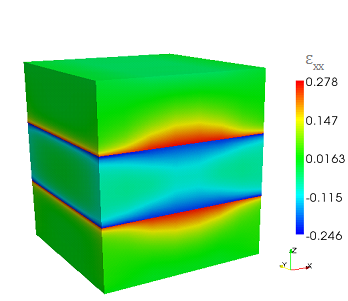
\includegraphics{elasticity01.png}
\label{Elasticity:fig-elasticity01}\end{figure}
\begin{figure}[htbp]
\centering

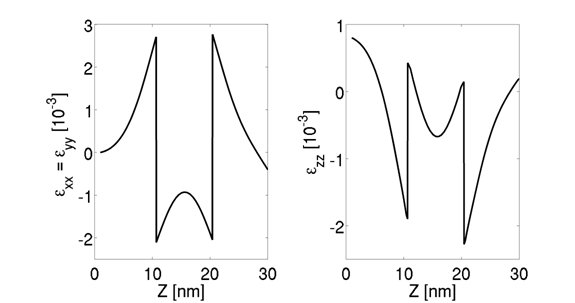
\includegraphics{elasticity02.png}
\label{Elasticity:fig-elasticity02}\end{figure}

Theoretical background


TiberCAD? computes the mechanical deformation of a body subjected to external forces by means of the equilibrium mechanical equation, i.e.

 \[
 \frac{\partial \sigma_{ij}}{\partial x_j} = f_i
 \]
wheres is the stress second-rank tensor and f is the external body force applied to the system.
As we will see below, any strain and stress source can be appropriately mapped into an equivalent body force.


The stress tensor e is related to the mechanical strain by means of the constitutive relationships $\sigma_{ij}=C_{ijlk}\epsilon_{lk}$
where \textbf{C} is the stiffness fourth-rank tensor.
The strain is related to the displacement u by the expression

 \[
 \epsilon_{kl}=\frac{1}{2}\left(\frac{\partial u_l}{x_k}-\frac{\partial u_k}{\partial u_l} \right )
 \]
Relying on the symmetry of the strain and stiffness tensor the final equation reads as

 \[
 \frac{\partial}{\partial x_j}C_{ijlk}\frac{\partial u_l}{\partial x_k} = f_i
 \]
The non-linear strain is computed by applying the mechanical equilibrium equation on the deformed mesh.
The number of the shape iteration is set by the keyword shape\_iteration (default = 0, i.e. no deformation is performed)
whereas the maximum tolerated error can be indicated with shape\_error (default = 1e-3).


Stiffness constant


By default the stiffness constant is anisotropic. For the zincoblend crystal structure the independent coefficients are
(with the Voigt notation) C11, C12, C44. For the wurtzite structure we have C11, C12, C13 and C44.An isotropic stiffness
can be included with the keyword Stiffness isotropic. In this case, the only independent parameters are the Young modulus
(Youngin GPa) and the Poisson?s ratio (Poisson).


Example:


\begin{Verbatim}[commandchars=@\[\]]
Stiffness isotropic
  {
   Young = 129
   Poisson = 0.349
  }
\end{Verbatim}

Boundary conditions:


Surfaces forces $f^0$ are applied by imposing $\sigma_{ij} n_{j} = f_i^0$ along the surface with normal n.
This boundary condition can be used with the keyword surface\_force. The force can be specified in GPa with force.
An example is shown below


\begin{Verbatim}[commandchars=@\[\]]
Contact base
  {
   type = surface@_force
   force = (0,0,0.5)
  }
\end{Verbatim}

On the other hand, one may want to fix some surface of the device. The keyword clamp freezes all nodes of a given surface.


Example:


\begin{Verbatim}[commandchars=@\[\]]
Contactsubstrate
  {
   type = clamp
  }
\end{Verbatim}

Body forces


A constant value body force can be included by means of the keyword Body\_force constant.


Example:


\begin{Verbatim}[commandchars=@\[\]]
BodyForceconstant
  {
   force = (0,1,0)
  }
\end{Verbatim}

When two crystals with different crystal structure are put in contact the lattice mismatch between them may induce a strain e\textasciicircum{}LM and, therefore, a stress s=?Ce?\textasciicircum{}LM.


This stress contribution acts as a body force

 \[
 f_i = -\frac{\partial }{\partial x_j} C_{ijlk}\epsilon_{lk}^{LM}
 \]
The strain source can be computed only once the reference lattice is identified.
The reference material and its growth axis can be included following the same syntax of the device section.


Example:


\begin{Verbatim}[commandchars=@\[\]]
BodyForcelattice@_mismatch
  {
   reference@_material = AlGaN
   structure = wz
   x = 0.2
   x-growth-direction = (1,0,0,0)
   y-growth-direction = (0,1,-1,0)
   z-growth-direction = (0,0,0,1)
  }
\end{Verbatim}

In presence of an electric field there might develop an additional stress source due to the so-called converse piezoelectric effect, given by :

 \[
 \sigma_{il}^{SC}=-e_{ijk}E_k
 \]
The converse piezoelectric effect can be included with the keyword BodyForcepiezo and an electrostatic simulation must be indicated.


The effective body force reads as :

 \[
 f_i = -\frac{\partial}{\partial x_j} \sigma_{ij}^{CP}
 \]
Example:


\begin{Verbatim}[commandchars=@\[\]]
BodyForceconverse@_piezo
  {
   poisson@_simulation = dd
  }
\end{Verbatim}

Considering all the above mentioned force sources, the plotted total stress and strain are :

 \[
 \sigma_{ij} = C_{ijlk}\left( \frac{\partial u_l}{\partial x_k} + \epsilon_{lk}^{LM} \right) -e_{ijk}E_k
 \] \[
 \epsilon_{kl}=\frac{1}{2}\left(\frac{\partial u_l}{x_k}-\frac{\partial u_k}{\partial u_l} \right ) + \epsilon_{lk}^{LM}
 \]
Reference Manual


Stiffness/Isotropic
Kind: bulk
Name: Stiffness
Type: isotropic
database\_section: none
Options:
young  (double,0.0)
poisson (double {[}-0.5,1.0{]},0.0)


Stiffness/Anisotropic
Kind: bulk
Name: Stiffness
Type: anisotropic
database\_section = stiffness
Options:
none


Body Force/constant
Kind: bulk
Name: BodyForce
Type: constant
database\_section: none
Options:
force (double vector,(0.0,0.0,0.0))


Body Force/Lattice Mismatch
Kind: bulk
Name: BodyForce
Type: lattice\_mismatch
database\_section: none
Options:
x (double {[}0.0,1,0{]},0.0)
x-growth-direction (double vector)
y-growth-direction (double vector)
z-growth-direction (double vector)


Body Force/Converse
Kind: bulk
Name: BodyForce
Type: converse
database\_section: piezoelectricity
Options:
poisson\_simulation (string,?none?)


Boundary/clamp
Kind: interface
Name: Contact
Type: converse
database\_section: none
Options:
poisson\_simulation (string,?none?)


Boundary/Surface Force
Kind: interface
Name: Contact
Type: surface\_force
database\_section: none
Options:
force (double vector,(0.0,0.0,0.0)



\chapter{Simulation Dye Solar Cells}
\label{Dsc:simulation-dye-solar-cells}\label{Dsc::doc}\label{Dsc:dsc}
For a brief list of literature to understand Dye Solar cells (DSC) see {\hyperref[Bibliography:kalyanasundaram]{{[}Kalyanasundaram{]}}} . For a review
of the model see {\hyperref[Bibliography:gagliardi]{{[}Gagliardi{]}}} .


The model consists in a set of drift-diflusion equations for the description of the
propagation of different ions and for the electrons coupled with Poisson equation:

\begin{eqnarray}
\nabla \cdot (\mu_{e}n_{e}\nabla\phi_{e}) & = & (G - R) \\
\nabla \cdot (\mu_{I^{-}}n_{I^{-}}\nabla\phi_{I^{-}}) & = & -\frac{3}{2}(G - R) \\
\nabla \cdot (\mu_{I^{-}_{3}}n_{I^{-}_{3}}\nabla\phi_{I^{-}_{3}}) & = & \frac{1}{2}(G - R) \\
\nabla \cdot (\mu_{c}n_{c}\nabla\phi_{c}) & = & 0,
\label{eq1}
\end{eqnarray}
where $\mu_\alpha$ refers to carrier mobilities, $n_\alpha$ to concentrations and $\phi_\alpha$ to electrochemical
potentials. \emph{R} is the recombination term and \emph{G} the generation term due to illumination.
The Poisson equation to handle the internal potential drop:

\begin{equation}\label{poisson}
-\varepsilon\triangle \varphi =  q[n_{c} + N_{D}^{+} - n_{I^{-}} - n_{I_{3}^{-}} - (n_{e} -
\bar{n}_{e})],
\end{equation}
where $N^+_D$ is the amount of ionized dyes and it is equal to:

\begin{equation}\label{dyeion}
N_{D}^{+} = \frac{G}{k_{3}}
\end{equation}
with \emph{G} the generation term and :math{}`k\_3{}` the rate constant of dye regeneration. The dielectric
constant, $\epsilon$ , of the mesoporous material is a mix the two dielectric functions of the semi-
conductor and the electrolyte. We use the Maxwell-Garnet model where the dielectric
function of the mixed medium becomes:

\begin{equation}\label{diel}
\varepsilon = \varepsilon_{s}\frac{\varepsilon_{e} + 2\varepsilon_{s} + 2\epsilon_{p}\varepsilon_{e} - 2\varepsilon_{s}\epsilon_{p}}
{\varepsilon_{e} + 2\varepsilon_{s} -\epsilon_{p}\varepsilon_{e} +\varepsilon_{s}\epsilon_{p}}
\end{equation}
where $\epsilon_s$ and $\epsilon_e$ are the dielectric constants of the semiconductor and the electrolyte,
respectively, and $\epsilon_p$ is the porosity of the medium. The recombination term depends
largely on the loss mechanisms at the electrolyte/oxide interface which follows the reac-
tion chain:

\begin{eqnarray}
I^{-} & \rightleftharpoons & I + e \\
2I & \rightleftharpoons & I_{2} \\
I_{2} + I^{-} & \rightleftharpoons & I^{-}_{3}.
\label{reaction_loss}
\end{eqnarray}
From the chemical path we can get a formula for the interface recombination (considering
that the flrst chemical reaction is the slow process):

\begin{equation}\label{ricombinazione}
R = k_{e} \left [  \left ( \frac{n_{e}}{\bar{n}_{e}} \right )^{\beta}\bar{n}_{e}\sqrt{\frac{n_{I^{-}_{3}}}{n_{I^{-}}}}
- \bar{n}_{e}\sqrt{\frac{\bar{n}_{I^{-}_{3}}}{\bar{n}^{3}_{I^{-}}}} n_{I^{-}}\right
],
\end{equation}
where the electron rate $k_e$ is the recombination rate constant.


For the boundary conditions of the model we assume at the photoanode:
*  $\phi_{e} = V$ : electrochemical potential of electrons set with the voltage applied;
*  $\nabla\phi_{I^{-}}  = 0$ : no iodide current at the photoande;
*  $\nabla\phi_{I_{3}^{-}} = 0$ : no triiodide current at the photoande;
*  $\nabla\phi_{c} = 0$ : no cationic current;
*  $\nabla\varphi = 0$ : no charged layer at the photoanode;


at the cathode:

\begin{itemize}
\item {} 
$\nabla\phi_{e} = 0$ : no electronic current at the cathode;


\item {} 
$-q\mu_{I^{-}}n_{I^{-}} \nabla\phi_{I^{-}} = \frac{3}{2}\left ( \frac{ - E_{red}(\mathbf{r_{c}})}{R_{L}} \right )$ : split of the current between the ionic species;


\item {} 
$-q\mu_{I^{-}_{3}} n_{I^{-}_{3}}\nabla\phi_{I^{-}_{3}} =  -\frac{1}{2}\left ( \frac{ - E_{red}(\mathbf{r}_{c})}{R_{L}} \right )$ : split of the current between the ionic species;


\item {} 
$\nabla\phi_{c} = 0$ : no cationic current;


\end{itemize}

integral boundary conditions for conservation of ionic species:

\begin{itemize}
\item {} 
$\int_{\Omega}$ $\left [ \frac{1}{3}n_{I^{-}}(\mathbf{r}) + n_{I^{-}_{3}}(\mathbf{r}) \right ] d\mathbf{r} = \left (\frac{1}{3}\bar{n}_{I^{-}} + \bar{n}_{I^{-}_{3}} \right )\Omega$ : conservation of iodine ions within the cell;


\item {} 
$\int_{\Omega} n_{c}(\mathbf{r}) d\mathbf{r}  =  \bar{n}_{c}\Omega$ : conservation of cation within the cell;


\end{itemize}

where $\omega$ is the volume of the cell, $n\alpha$ the density of charged species and the index $\alpha$
stands for cation (c), iodide ( $I^{-}$ ), triiodide ( $I^{-}_3$ ) and electrons (e). $R_L$ is the external
load. The bias applied is equal to:

\begin{equation}\label{pot1}
V = \phi_{e} - E_{red}.
\end{equation}
$E_{red}$ is the redox potential. The redox potential can be evaluated using a Nernst approx-
imation:

\begin{equation}\label{pot1}
V = \phi_{e} - E_{red}.
\end{equation}\phantomsection\label{Bibliography:bibliography}
\begin{thebibliography}{Kalyanasundaram}
\bibitem[Kalyanasundaram]{Kalyanasundaram}{\phantomsection\label{Bibliography:kalyanasundaram} 
Kalyanasundaram Kuppuswamy, ``Dye-Sensitized Solar Cells'', \emph{Editor Crc Pr Inc.} , 2010.

}
\bibitem[Gagliardi]{Gagliardi}{\phantomsection\label{Bibliography:gagliardi} 
Alessio Gagliardi, Matthias Auf der Maur, Desiree Gentilini and Aldo Di Carlo, ``Modeling of Dye sensitized solar cells using a finite element method'',
\emph{J. Computational Electronics} , vol. 8, pp. 12, 2009.

}
\end{thebibliography}



\renewcommand{\indexname}{Index}
\printindex
\end{document}
